\documentclass[a4paper,norsk]{article}
\usepackage[utf8]{inputenc}
\usepackage[T1]{fontenc,url}
\usepackage{babel,textcomp}
\usepackage{graphicx}
\usepackage{amsmath}
\usepackage{cleveref}
\usepackage[cmyk]{xcolor}
\usepackage{listings}
\graphicspath{ {./images/} }
\lstset {language=C++,    
backgroundcolor=\color{yellow!20},    
commentstyle=\color{green},    
%keywordstyle=\color{blue},    
basicstyle=\footnotesize}
\urlstyle{sf}
\title{Matte 3 Oblig 2}
\date{\today}
\author{Sivert Kindberg}
\newpage
\begin{document}
\maketitle
\tableofcontents
\newpage
 \section{Github}


\section{Oppgave 3.4.6}
Oppgave 3.4.6
utregningene er gjort i Excel \newline
Valgte punkter: (3, 10), ( 1, 6.5), (-5.9, 7.6), (-3, 5), (-2, 1.7), (-7, 4.3), (6.9, 4.2), (3.8, 5.2)\newline
\newline
y = Ax + e 
\newline
\begin{equation*} 
\begin{bmatrix}10 \\ 6.5\\7.6\\5\\1.7\\4.3\\4.2\\5.2\end{bmatrix}
=\begin{bmatrix}9 & 3 & 1 \\ 1 & 1 & 1 \\34.81 & -5.9 & 1 \\ 9 & -3 & 1 \\4 & -2 & 1 \\49& 7 & 1 \\47.61 & 6.9 & 1 \\ 14.9 & 3.8 & 1\end{bmatrix}\begin{bmatrix}a\\b\end{bmatrix}
+ \begin{bmatrix} e_1 \\ e_2 \\ e_3 \\ e_4 \\ e_5 \\ e_6 \\ e_7\end{bmatrix}
\end{equation*}


\begin{equation*}
B = A^{T} * A = \begin{bmatrix} 9 & 1 & 34.81 & 9 & 4 & 49 & 47.61 & 14.9 \\  3 & 1 & -5.9 & -3 & -2 & 7 & 6.9 & 3.8 \\1 & 1 & 1 & 1& 1 & 1 & 1 & 1\end{bmatrix}
\begin{bmatrix}  9 & 3 & 1 \\ 1 & 1 & 1 \\ 34.81 & -5.9 & 1 \\  9 & -3 & 1 \\4 & -2 & 1  \\49 & 7 & 1 \\47.61 & 6.9 & 1 \\ 14.9 & 3.8 & 1\end{bmatrix}
=\begin{bmatrix} 6280.4582 & 515.75 & 169.32 \\ 515.75 & 168.86 & 10.8 \\ 169.32 & 10.8 & 8\end{bmatrix}
\end{equation*} 


\begin{equation*}
C = A^{T} * y = \begin{bmatrix} 9 & 1 & 34.81 & 9 & 4 & 49 & 47.61 & 14.9 \\  3 & 1 & -5.9 & -3 & -2 & 7 & 6.9 & 3.8 \\1 & 1 & 1 & 1& 1 & 1 & 1 & 1 \end{bmatrix}
\begin{bmatrix}10 \\ 6.5\\7.6\\5\\1.7\\4.3\\4.2\\5.2\end{bmatrix}
=\begin{bmatrix}900.998 \\52.1 \\44.5 \end{bmatrix}
\end{equation*}

\begin{equation*}
B^{-1} = \begin{bmatrix} 0.000462474 & -0.000860823 & -0.008626157\\ -0.000860823 & 0.008084009 & 0.007305914 \\-0.008626157 & 0.007305914 & 0.297709637  \end{bmatrix}
\end{equation*}


\begin{equation*}
x = B^{-1} * c = \begin{bmatrix}  6280.4582 & 515.75 & 169.32 \\ 515.75 & 168.86 & 10.8 \\ 169.32 & 10.8 & 8  \end{bmatrix}\begin{bmatrix} 900.998 \\52.1 \\44.5 \end{bmatrix}
= \begin{bmatrix}-0.012024466 \\ -0.029310073 & 5.856566423 \end{bmatrix}
\end{equation*}

$y =-0.012024466x^{2}-0.029310073x+5.856566423$
\section{Beregne punkter og lagre i array}
Funksjonen tar inn x som verdi og bruker funksjonen fra utergningen og returnerer y verdien punktet skal ha.
\begin{lstlisting}[language=C++, caption={trianglesurface.h}]
static float func2(float x) {
       return 0.174 * x + 1, 743;
   }
\end{lstlisting}
\section{3.4.6 Visualisering}
VisualPoint klassen tar inn en vector av Vertexer, vertexene blir vist som hvite kvadrater.. MMap får en QuadraticPolynomial som tegner den grønne kurven.
\begin{lstlisting}[language=C++, caption={renderwindow.cpp}]
    mMap.insert(std::pair<std::string, VisualObject*>{"QuadtraticPolynomial", new QuadtraticPolynomial(-0.012024466, -0.029310073f, 5.856566423f, 0.1f)});
    std::vector<Vertex> points;
    points.push_back(Vertex{ 3, 10, 0 });
    points.push_back(Vertex{ 1, 6.5, 0 });
    points.push_back(Vertex{ -5.9, 7.6, 0 });
    points.push_back(Vertex{ -3, 5, 0 });
    points.push_back(Vertex{ -2, 1.7, 0 });
    points.push_back(Vertex{ -7, 4.3, 0 });
    points.push_back(Vertex{ 6.9, 4.2, 0 });
    points.push_back(Vertex{ 3.8, 5.2, 0 });

    for (auto i = 0; i < points.size(); i++) 
    {
        mMap.insert(std::pair<std::string, VisualObject*>
{ std::to_string(i), new VisualPoint(points)});
    }
    
\end{lstlisting}
\centering
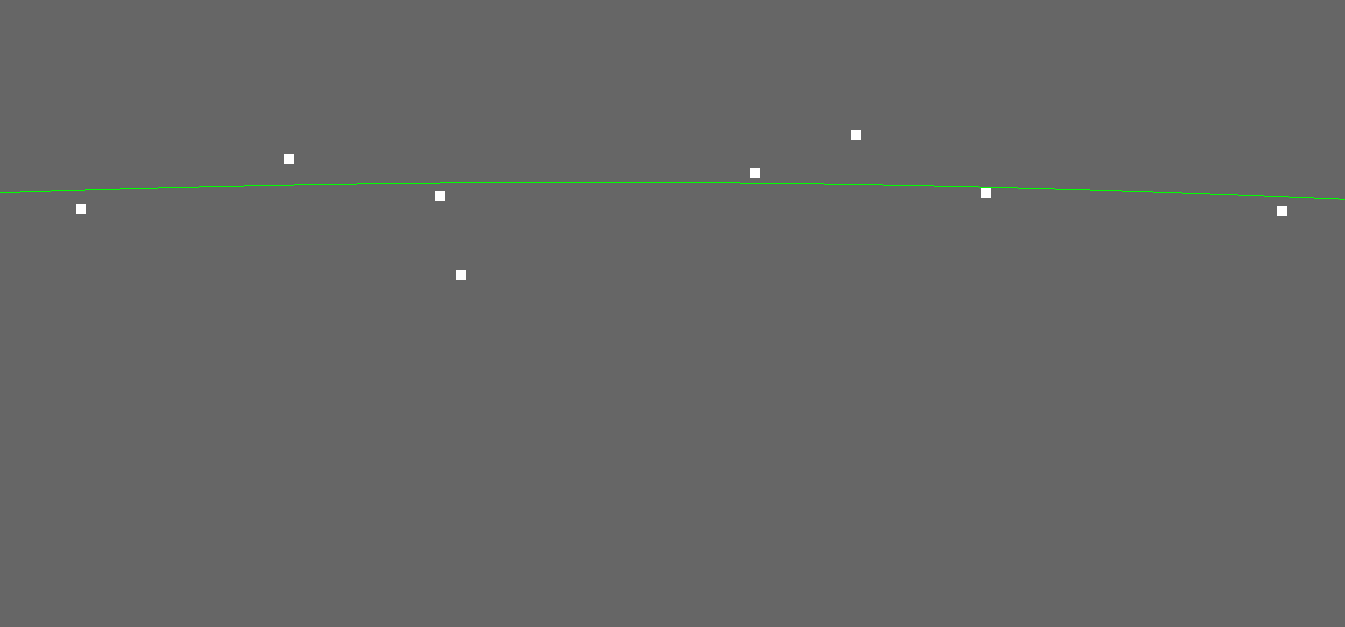
\includegraphics[width=\textwidth]{kurve1}


\section{Oppgave 4.6.7}
Punkter: ( 0.9, 0.6), ( 2.6, -1.1), (3.5, 3.7), (6.9, 4.2) 
\newline

\begin{equation*}
A = \begin{bmatrix} 0.729  & 0.81 & 0.9 & 1 \\  17.576 & 6.76 & 9.9 & 1 \\  42.875 & 12.25 & 3.9 & 1 \\  328.509 & 47.61 & 6.9 & 1 \end{bmatrix} B = \begin{bmatrix} 0.6 \\ -1.1 \\ 3.7 \\ 4.2 \end{bmatrix}\end{equation*}
\newline
\begin{equation*}
A^{-1} = \begin{bmatrix} 0.017779746 & 0.005580521 & -0.029978972 & 0.006618704 \\  -0.139178717 & -0.056805602 & 0.221551832 & -0.025567513 \\ 
 -0.052380225 & 0.13821981 & -0.090353074 & 0.004513489 \\  1.146915528 & -0.082453491 & -0.076284547 & 0.01182251 \end{bmatrix}
\end{equation*}
\newline
$x = A^{-1}*B = $
\begin{equation*}
\begin{bmatrix} 0.017779746 & 0.005580521 & -0.029978972 & 0.006618704 \\  -0.139178717 & -0.056805602 & 0.221551832 & -0.025567513 \\ 
 -0.052380225 & 0.13821981 & -0.090353074 & 0.004513489 \\  1.146915528 & -0.082453491 & -0.076284547 & 0.01182251  \end{bmatrix} \begin{bmatrix}   0.6 \\ -1.1 \\ 3.7 \\ 4.2 \end{bmatrix}
\newline
= \begin{bmatrix}  -0.078594 \\  0.691337 \\-0.498819 \\  0.546249 \end{bmatrix} 
\newline
\newline
f(x) = -0.78x^{3} + 0,69x^{2}-0,49x + 0,54
\end{equation*}

\section{4.6.7 Visualisering}

her bruker jeg cubicpolimal for å sette punktene;
\begin{lstlisting}[language=C++, caption={cubicpolynomial.cpp}]
CubicPolynomial::CubicPolynomial(double a, double b, double c, double d, float dx)
{
   
    for (auto x = -10.f; x <= 10; x += 0.1)
    {
        auto y = p(a, b, c, d, x);
        mVertices.push_back(Vertex(x, y, 0, 0, 1, 0));
    }
    mMatrix.setToIdentity();

}

double CubicPolynomial::p(double a, double b, double c, double d, double x)
{
    return a * x * x * x + b * x * x + c * x + d;
\end{lstlisting}
\begin{lstlisting}[language=C++, caption={renderwindow.cpp}]
    mMap.insert(std::pair<std::string, VisualObject*>{"CubicPolynomial", new CubicPolynomial(-0.78, 0.69, -0.49, 0.54, 0.1f)});
    std::vector<Vertex> points2;
    points2.push_back(Vertex{ 0.9f, 0.6f, 0 });
    points2.push_back(Vertex{ 2.6f, -1.1f, 0 });
    points2.push_back(Vertex{ 3.5f, 3.7f, 0 });
    points2.push_back(Vertex{ 6.9f, 4.2, 0 });

    for (auto i = 0; i < points2.size(); i++) 
    {
        mMap.insert(std::pair<std::string, VisualObject*>{ std::to_string(i * 10), new VisualPoint(points2)});
    }
\end{lstlisting}

\centering
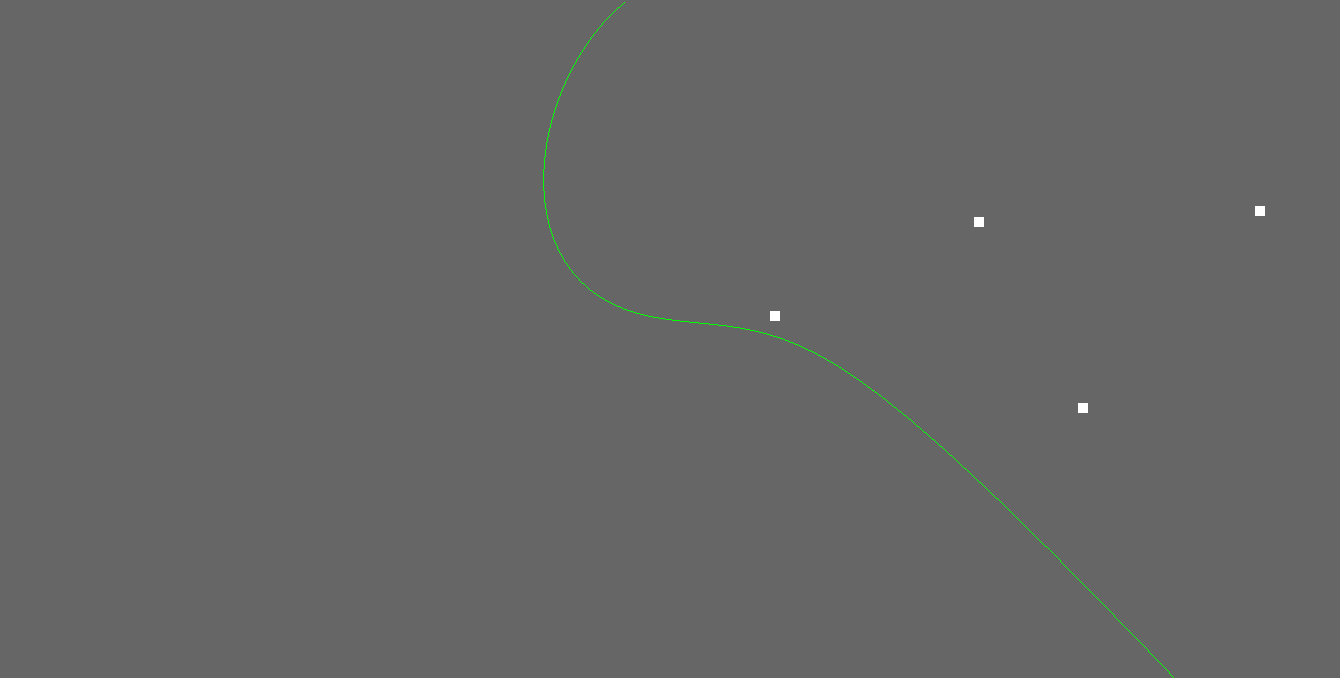
\includegraphics[width=\textwidth]{kurve2}
ser ikke riktig ut, er ganske sikker på at utregningen er riktig, kan være metodikkebn eller koden

\section{Oppgave 4.11.6}
Bezier kurve

\begin{lstlisting}[language=C++, caption={beziercurve.h}]
#ifndef BEZIERCURVE_H
#define BEZIERCURVE_H

#include "visualobject.h"
#include "visualpoint.h"
#include <vector>
class BezierCurve : public VisualObject
{
public:
	BezierCurve(std::vector<QVector3D> controlPoints);
	void init(GLint matrixUniform) override;
	void draw() override;
	int d = 3;
private:
	std::vector<QVector3D> mControlPoints;
	std::vector<Vertex> mControlPointsVertices;
	VisualPoint* mControlPointVisual;
	QVector3D EvaluateBezier(float t);
};

#endif // BEZIERCURVE_H
\end{lstlisting}
\begin{lstlisting}[language=C++, caption={beziercurve.cpp}]
#include "beziercurve.h"

BezierCurve::BezierCurve(std::vector<QVector3D> controlPoints) 
{
    mControlPoints = controlPoints;
    //Create vertexs from control points
    for (auto it : mControlPoints) 
    {
        mControlPointsVertices.push_back(Vertex(it.x(), it.y(), it.z(), 1.f, 1.f, 1.f));
    }
    //Visualpoint for displaying control points
    mControlPointVisual = new VisualPoint(mControlPointsVertices);

    for (float t{}; t < 1.00f; t += 0.01f) 
    {
        QVector3D point = EvaluateBezier(t);

        mVertices.push_back(Vertex(point.x(), point.y(), point.z()));
    }
}

void BezierCurve::init(GLint matrixUniform)
{
    mMatrixUniform = matrixUniform;
    initializeOpenGLFunctions();

    glGenVertexArrays(1, &mVAO);
    glBindVertexArray(mVAO);

    // Vertex buffer object(VBO), holding vertices
    glGenBuffers(1, &mVBO);
    glBindBuffer(GL_ARRAY_BUFFER, mVBO);
    glBufferData(GL_ARRAY_BUFFER,
        mVertices.size() * sizeof(Vertex),
        mVertices.data(),
        GL_STATIC_DRAW
    );

    // Vertices
    glBindBuffer(GL_ARRAY_BUFFER, mVBO);
    glVertexAttribPointer(
        0,
        3,
        GL_FLOAT,
        GL_FALSE,
        sizeof(Vertex),
        reinterpret_cast<GLvoid*>(0));
    glEnableVertexAttribArray(0);

    // Colors
    glVertexAttribPointer(
        1,
        3,
        GL_FLOAT,
        GL_FALSE,
        sizeof(Vertex),
        reinterpret_cast<GLvoid*>(3 * sizeof(GLfloat))
    );

    glEnableVertexAttribArray(1);

    glBindVertexArray(0);

    if (mControlPointVisual)
        mControlPointVisual->init(matrixUniform);
}

void BezierCurve::draw() 
{
    initializeOpenGLFunctions();

    glBindVertexArray(mVAO);
    glUniformMatrix4fv(mMatrixUniform, 1, GL_FALSE, mMatrix.constData());
    glDrawArrays(GL_LINE_STRIP, 0, mVertices.size());

    if (mControlPointVisual)
        mControlPointVisual->draw();
}

QVector3D BezierCurve::EvaluateBezier(float t)
{
    std::vector<QVector3D> temp;

    //Gets the control points
    for (int i = 0; i < mControlPoints.size(); i++)
    {
        temp.push_back(mControlPoints[i]);
    }
    for (int k = temp.size() - 1; k > 0; k--)
    {
        for (int i = 0; i < k; i++)
            //Bezier algoritmen
            temp[i] = temp[i] * (1 - t) + temp[i + 1] * t;
    }
    return temp[0];
}
\end{lstlisting}
\begin{lstlisting}[language=C++, caption={renderwindow.cpp}]
    std::vector<QVector3D> controlPoints;
    controlPoints.push_back(QVector3D(0.f, 0.f, 0.f));
    controlPoints.push_back(QVector3D(2.f, 3.f, 0.f));
    controlPoints.push_back(QVector3D(4.f, -3.f, 0.f));
    controlPoints.push_back(QVector3D(6.f, 3.f, 0.f));
    mMap.insert(std::pair<std::string, VisualObject*>{"BezierCurve", new BezierCurve(controlPoints)});
\end{lstlisting}
bilde av kurven:
\centering
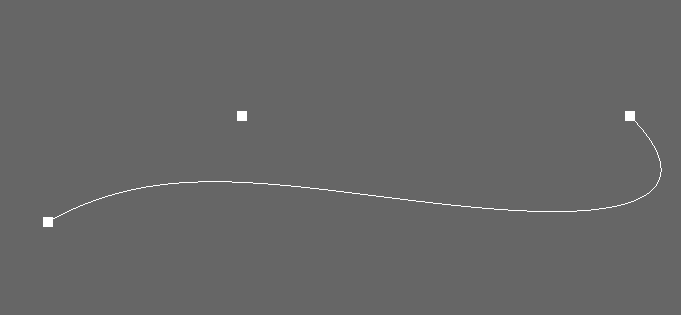
\includegraphics[width=\textwidth]{kurve3}
\end{document}